\chapter{Related Work}

\section{CTR Prediction}

Current click-through rate (CTR) prediction methods can be categorized into two main types: \textit{feature engineering} and \textit{model engineering}.

\subsection{Feature Engineering}

Feature engineering focuses on mining and selecting informative features relevant to CTR prediction. These features include graph features, visual features, textual features, and multimodal features. For example, some methods collect textual descriptions of features, encode the text using pretrained language models (PLMs) to obtain semantic embeddings, and employ alignment loss to align collaborative signals with these embeddings.

Several studies have also focused on filtering out noisy or irrelevant features using automated selection or attention-based methods~\cite{liu2020autofis, liu2024multifs}.

\subsection{Model Engineering}

Model engineering aims to design more effective models to extract information from the input features. This includes developing diverse types of feature interactions, such as Factorization Machines (FM)~\cite{rendle2010factorization}, DeepFM~\cite{guo2017deepfm}, EulerNet~\cite{tian2023eulernet}, and KAN~\cite{shi2024beyond}.

In addition, many works model user interests—especially long- and short-term interests—based on behavior sequences~\cite{zhou2018deep, zhou2019deep}. These techniques aim to dynamically capture evolving user preferences and improve recommendation quality.

This study falls under the category of feature engineering. Specifically, we mine multi-faceted knowledge from entangled textual information and integrate this knowledge into CTR prediction.

\subsection{Comprehensive Comparison of CTR Methods}

To better understand the landscape of CTR prediction, we provide a detailed comparison of representative methods across different categories:

\begin{table}[htbp]
\centering
\caption{Comprehensive Comparison of CTR Prediction Methods}
\label{tab:ctr-comparison}
\resizebox{\textwidth}{!}{
\begin{tabular}{l|c|c|c|c|c}
\toprule
\textbf{Method} & \textbf{Category} & \textbf{Feature Type} & \textbf{Interaction Order} & \textbf{Text Support} & \textbf{Complexity} \\
\midrule
LR & Traditional & Categorical & 1st & No & Low \\
FM & Traditional & Mixed & 2nd & No & Medium \\
FFM & Traditional & Mixed & 2nd & No & Medium \\
Wide \& Deep & Deep Learning & Mixed & Mixed & Limited & Medium \\
DeepFM & Deep Learning & Mixed & Mixed & Limited & Medium \\
DCN & Deep Learning & Mixed & High-order & Limited & High \\
DCNv2 & Deep Learning & Mixed & High-order & Limited & High \\
DIN & Attention-based & Sequential & Mixed & No & Medium \\
DIEN & Attention-based & Sequential & Mixed & No & High \\
BERT4CTR & PLM-based & Mixed + Text & Mixed & Yes & Very High \\
CTRL & PLM-based & Mixed + Text & Mixed & Yes & Very High \\
MSD-CTR (Ours) & Disentangled & Mixed + Text & Mixed & Yes & High \\
\bottomrule
\end{tabular}
}
\end{table}

The comparison reveals several key insights:
\begin{itemize}
    \item \textbf{Evolution Trend}: Methods have evolved from simple linear models to complex neural architectures incorporating attention mechanisms and pre-trained language models.
    \item \textbf{Text Integration}: Recent methods increasingly leverage textual information, but most suffer from entangled semantic representations.
    \item \textbf{Complexity Trade-off}: Higher model complexity generally improves performance but increases computational overhead and deployment challenges.
    \item \textbf{Feature Interaction}: Advanced methods focus on learning sophisticated feature interactions, from 2nd-order (FM) to arbitrary high-order (DCN).
\end{itemize}

\section{PLM Integration and Multimodal Trends in Recommendation}

The integration of Pre-trained Language Models (PLMs) into recommendation systems represents a significant paradigm shift, driven by their exceptional ability to understand and encode semantic information from textual content.

\subsection{Evolution of PLM-based Recommendation}

\textbf{First Generation (2019-2020):} Early attempts focused on using BERT embeddings as additional features. Methods directly fine-tuned BERT~\cite{devlin2019bert} for recommendation tasks, achieving modest improvements over traditional methods.

\textbf{Second Generation (2021-2022):} More sophisticated integration strategies emerged. Advanced methods applied bidirectional self-attention to model user sequences, while others unified different recommendation scenarios under pre-trained frameworks.

\textbf{Third Generation (2023-Present):} Current approaches focus on addressing specific challenges in PLM-recommendation integration:
\begin{itemize}
    \item \textbf{Domain Adaptation}: Methods address the domain gap between pre-training corpora and recommendation scenarios.
    \item \textbf{Efficiency Optimization}: Techniques like knowledge distillation and parameter-efficient fine-tuning reduce computational overhead while maintaining performance.
    \item \textbf{Multimodal Fusion}: Advanced architectures combine textual, visual, and behavioral signals for comprehensive user understanding~\cite{wang2021multimodal}.
\end{itemize}

\subsection{Multimodal Recommendation Systems}

Modern recommendation systems increasingly incorporate multiple modalities beyond traditional collaborative filtering signals:

\textbf{Text-Visual Fusion:} Methods combine textual descriptions with visual features from product images~\cite{liu2020category, yu2022boost}. However, these approaches often suffer from modality imbalance, where one modality dominates the learned representations.

\textbf{Text-Audio Integration:} In music and video recommendation, audio features provide complementary information to textual metadata. Recent work explores attention-based fusion mechanisms to balance different modalities effectively.

\textbf{Temporal Dynamics:} Advanced systems model how multimodal preferences evolve over time~\cite{zhou2024temporal}. Methods use self-supervised learning to capture temporal patterns across modalities.

\subsection{Generative Models in Recommendation}

The success of large language models has sparked interest in generative approaches to recommendation:

\textbf{Language Model-based Recommendation:} Methods frame recommendation as a text generation task, leveraging the reasoning capabilities of large language models~\cite{rajput2023recommender}.

\textbf{Diffusion Models:} Recent work explores diffusion models for recommendation, treating user preferences as a denoising process. These methods show promise for handling uncertainty and generating diverse recommendations.

\textbf{Hybrid Generative-Discriminative:} Approaches combining generative and discriminative paradigms offer balanced performance, leveraging the strengths of both methodologies while mitigating their individual limitations.

\section{Disentangled Representation Learning}

Disentangled representation learning (DRL) seeks to extract informative and independent factors of variation in data. It has gained significant attention due to its superior explainability~\cite{wang2024disentangled}.

\subsection{VAE-based Disentanglement}

VAE-based DRL methods can be divided into:
\begin{itemize}
    \item \textbf{Unsupervised approaches}, which re-weight or decompose the evidence lower bound (ELBO) of the VAE to encourage factor separation~\cite{higgins2017beta, burgess2018understanding}.
    \item \textbf{Supervised approaches}, which introduce weak supervision signals such as grouping or causal relationships to enforce disentanglement~\cite{yang2021causalvae}.
\end{itemize}

\subsection{DRL in Recommendation}

DRL for recommendation systems aims to enhance representation learning by separating latent aspects such as:
\begin{itemize}
    \item User interests (e.g., short-term vs. long-term)~\cite{ma2019learning, ma2020disentangled}.
    \item Multi-source inputs (e.g., user-item interaction vs. side information)~\cite{wang2020disentangled}.
\end{itemize}

Compared to existing studies, our method focuses on disentangling semantic embeddings from textual side information and using the learned factors to guide CTR prediction.

\section{Topic Model Evolution and Neural Approaches}

Traditional topic models aim to discover latent semantic structures in document collections using probabilistic graphical models (e.g., LDA, dynamic topic models). These models typically infer topic-word and document-topic distributions using methods such as Gibbs sampling or variational inference.

\subsection{Classical Topic Models: From LDA to Advanced Variants}

\textbf{Latent Dirichlet Allocation (LDA):} Introduced by Blei et al.~\cite{blei2003latent}, LDA remains the foundational topic model. It assumes each document is a mixture of topics, where each topic is characterized by a distribution over words. The generative process follows:
\begin{enumerate}
    \item For each topic $k$: Draw word distribution $\phi_k \sim \text{Dir}(\beta)$
    \item For each document $d$: Draw topic distribution $\theta_d \sim \text{Dir}(\alpha)$
    \item For each word position: Draw topic $z \sim \text{Cat}(\theta_d)$, then word $w \sim \text{Cat}(\phi_z)$
\end{enumerate}

Despite its popularity, LDA suffers from several limitations: (1) inability to capture word order and semantic relationships, (2) difficulty in determining optimal topic numbers, and (3) computational scalability issues for large corpora.

\textbf{Dynamic Topic Models:} To address temporal evolution, dynamic topic models~\cite{blei2006dynamic} model how topics change over time slices. The Continuous Time Dynamic Topic Model (cDTM) further enables modeling of arbitrary time intervals.

\textbf{Hierarchical Topic Models:} The Hierarchical Dirichlet Process (HDP) automatically determines the number of topics, while Pachinko Allocation Models model correlations between topics through directed acyclic graphs.

\subsection{Neural Topic Models: Bridging Deep Learning and Topic Modeling}

With the success of VAE, neural topic models emerged, which combine the reparameterization trick with BoW-based document representation~\cite{srivastava2017autoencoding}.

\textbf{Neural Variational Document Model (NVDM):} One of the first neural topic models, NVDM uses a VAE framework to learn document representations. However, it lacks explicit topic interpretability compared to traditional models.

\textbf{Embedded Topic Model (ETM):} ETM~\cite{dieng2020topic} addresses interpretability by learning topic and word embeddings jointly. It factorizes the topic-word distribution as:
$$\beta = \text{softmax}(\alpha \rho^T)$$
where $\alpha$ represents topic embeddings and $\rho$ represents word embeddings in the same semantic space.

\textbf{Contextualized Topic Models:} Recent work leverages pre-trained language model embeddings to improve topic quality and enable zero-shot topic modeling across languages~\cite{wu2024fastopic}.

\subsection{BERTopic and Transformer-based Approaches}

\textbf{BERTopic Framework:} BERTopic~\cite{grootendorst2022bertopic} represents a paradigm shift by using transformer embeddings for initial document representation, followed by dimensionality reduction (UMAP) and clustering (HDBSCAN). This approach combines the semantic understanding of transformers with the interpretability of traditional topic models.

The BERTopic pipeline consists of:
\begin{enumerate}
    \item \textbf{Embedding Generation}: Use pre-trained transformers (BERT, RoBERTa, etc.) to encode documents
    \item \textbf{Dimensionality Reduction}: Apply UMAP to reduce embedding dimensions while preserving local structure
    \item \textbf{Clustering}: Use HDBSCAN to identify document clusters as topics
    \item \textbf{Topic Representation}: Extract representative words using TF-IDF within clusters
\end{enumerate}

\textbf{Advantages and Limitations:} While BERTopic achieves superior topic coherence and semantic quality, it faces several limitations: (1) lack of probabilistic interpretation, (2) difficulty in controlling topic granularity, and (3) computational overhead for large-scale applications.

\textbf{Recent Extensions:} Several variants address these limitations by introducing probabilistic topic assignments, enabling multi-level topic discovery, and supporting streaming document processing~\cite{wu2023effective}.

\section{Limitations Analysis and Research Motivation}

\subsection{Fundamental Limitations in Current Approaches}

Despite significant advances in text-enhanced CTR prediction, several fundamental limitations persist that motivate our research:

\textbf{Semantic Entanglement Problem:} Current PLM-based methods encode entire textual descriptions into single dense vectors, conflating distinct semantic aspects~\cite{wang2023bert4ctr, li2023ctrl}. For instance, a product description mentioning "premium leather quality" and "affordable price" contains contradictory semantic signals that become entangled in unified representations. This entanglement prevents models from understanding nuanced user preferences that may favor quality over price or vice versa.

\textbf{Limited Controllability:} Existing methods lack mechanisms to control which semantic aspects influence predictions. In real-world scenarios, different user segments may prioritize different aspects (price-sensitive vs. quality-focused), but current approaches cannot adapt representations accordingly.

\textbf{Scalability Challenges:} PLM integration introduces significant computational overhead~\cite{guo2024embedding}. BERT-large requires ~340M parameters and substantial memory, making real-time CTR prediction challenging for systems handling millions of requests per second. Current approaches lack efficient mechanisms to balance semantic understanding with computational constraints.

\textbf{Interpretability Gaps:} While PLMs capture rich semantic information, the learned representations remain largely opaque. This lack of interpretability hinders model debugging, bias detection, and business insight generation—critical requirements for production recommendation systems.

\subsection{Research Gap Analysis}

\textbf{Gap 1: Disentanglement in Recommendation Context:} While disentangled representation learning has shown promise in computer vision and natural language processing~\cite{locatello2019challenging}, its application to recommendation systems remains limited. Existing work focuses primarily on user-item interactions rather than semantic content disentanglement.

\textbf{Gap 2: Topic Model Integration:} Traditional topic models and modern deep learning approaches remain largely disconnected. Few methods effectively combine the interpretability of topic models with the expressiveness of neural networks for recommendation tasks.

\textbf{Gap 3: Multi-faceted Knowledge Utilization:} Current approaches fail to effectively leverage the multi-faceted nature of textual information~\cite{zhang2024towards}. Product descriptions contain diverse aspects (features, sentiment, brand positioning) that require specialized handling rather than uniform encoding.

\subsection{Motivation for Our Approach}

Our research is motivated by the need to address these fundamental limitations through a principled approach that:

\begin{enumerate}
    \item \textbf{Enables Semantic Disentanglement:} Develops mechanisms to separate entangled semantic aspects while maintaining their individual contributions to prediction tasks.
    
    \item \textbf{Provides Interpretable Representations:} Bridges topic modeling interpretability with deep learning expressiveness, enabling understanding of what semantic aspects drive predictions.
    
    \item \textbf{Ensures Computational Efficiency:} Designs approaches that balance semantic understanding with computational requirements for practical deployment.
    
    \item \textbf{Supports Multi-faceted Integration:} Creates frameworks that effectively utilize diverse semantic aspects rather than treating all textual information uniformly.
\end{enumerate}

\section{Real-world Applications and Deployment Considerations}

\subsection{Industry Applications and Case Studies}

\textbf{E-commerce Platforms:} Major e-commerce platforms handle billions of CTR prediction requests daily. These systems must balance recommendation quality with strict latency requirements (typically <100ms end-to-end). Text-enhanced CTR prediction becomes crucial for new product recommendations where collaborative filtering signals are sparse.

\textbf{Social Media Advertising:} Platforms leverage textual content from posts, comments, and user profiles for ad targeting. The challenge lies in processing dynamic, informal text content while maintaining user privacy and avoiding algorithmic bias.

\textbf{Video Streaming Services:} Streaming platforms use textual metadata (titles, descriptions, tags) combined with collaborative signals for content recommendation. The temporal nature of content consumption and the need for real-time personalization pose unique challenges.

\textbf{News and Content Platforms:} News recommendation systems must process article content, user reading history, and temporal trends to deliver relevant content. The rapid evolution of topics and the need for diversity make semantic understanding crucial.

\subsection{Deployment Architecture Considerations}

\textbf{Offline-Online Architecture:} Production systems typically employ a two-stage architecture:
\begin{enumerate}
    \item \textbf{Offline Stage:} Batch processing for computationally expensive operations like topic model training and semantic embedding generation.
    \item \textbf{Online Stage:} Real-time feature serving and lightweight model inference for user requests.
\end{enumerate}

\textbf{Scalability Requirements:} Large-scale systems must handle:
\begin{itemize}
    \item Millions of concurrent users
    \item Terabytes of textual data daily
    \item Sub-millisecond inference latency
    \item High availability (99.9%+ uptime)
\end{itemize}

\textbf{Infrastructure Challenges:} Deploying text-enhanced CTR systems requires:
\begin{itemize}
    \item Distributed computing frameworks for model training
    \item High-performance serving infrastructure for inference
    \item Efficient data pipelines for feature engineering
    \item Monitoring systems for model performance tracking
\end{itemize}

\section{Qualitative Study}

\subsection{Visualization of Learned Embeddings}

To evaluate the quality of the learned semantic representations, we visualize different models' embeddings using t-SNE~\cite{van2008visualizing}. We compare:
\begin{itemize}
    \item Disentangled topic embeddings from \textbf{DSTopic}.
    \item Disentangled semantic embeddings from \textbf{TopicDRL}.
    \item Naive concat embeddings.
    \item Other baseline methods.
\end{itemize}

\begin{figure}[htbp]
    \centering
    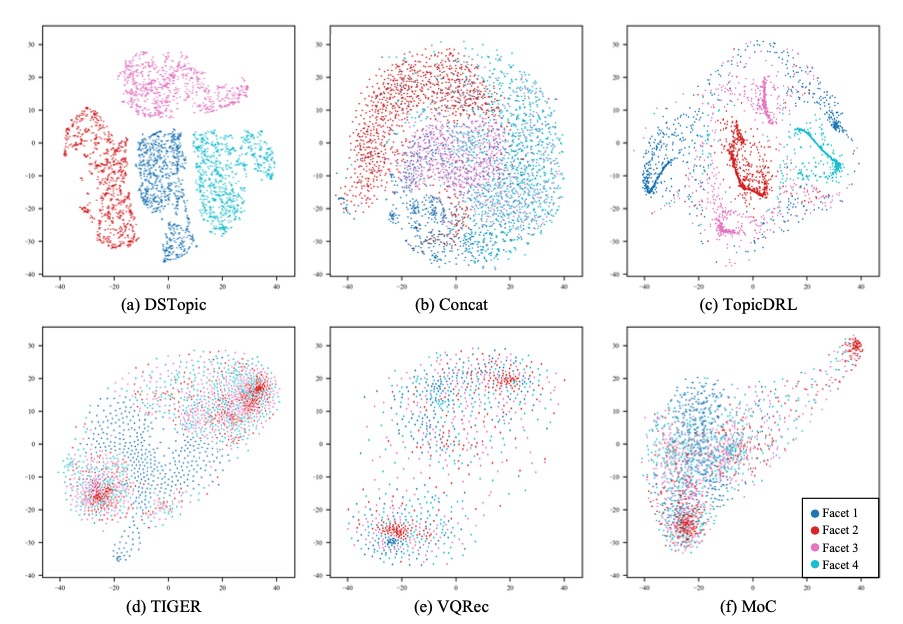
\includegraphics[width=\textwidth]{Figures/Chapter5/fig3.png}
    \caption{Visualization of learned semantic embeddings using DCNv2 on the Garden dataset.}
    \label{fig:tsne}
\end{figure}

The visualization reveals several key insights about the quality of learned representations:

\textbf{Cluster Separation:} DSTopic and TopicDRL demonstrate superior cluster separation compared to baseline methods. Each semantic view forms distinct clusters in the embedding space, indicating successful disentanglement of different semantic aspects.

\textbf{Semantic Coherence:} Within each cluster, semantically similar items group together, suggesting that our method preserves meaningful relationships while achieving disentanglement. For example, outdoor gardening tools cluster separately from indoor plant care products.

\textbf{Boundary Definition:} Clear boundaries between different semantic aspects indicate that our approach successfully avoids the entanglement problem that plagues concatenation-based methods.

\textbf{Dimensionality Efficiency:} The compact yet well-separated clusters suggest efficient use of the embedding space, avoiding the curse of dimensionality that often affects high-dimensional PLM embeddings.

\subsection{Interpretability Analysis}

\textbf{Topic Word Analysis:} We analyze the top words for each discovered topic to assess interpretability:

\begin{table}[htbp]
\centering
\caption{Sample Topic Words from DSTopic on Garden Dataset}
\label{tab:topic-words}
\begin{tabular}{l|l}
\toprule
\textbf{Topic/View} & \textbf{Top Words} \\
\midrule
Plant Care & watering, fertilizer, nutrients, growth, care, maintenance \\
Garden Tools & shovel, rake, pruning, cutting, digging, equipment \\
Outdoor Furniture & chair, table, patio, outdoor, weather, resistant \\
Seeds \& Plants & seeds, bulbs, flowers, vegetables, planting, growing \\
\bottomrule
\end{tabular}
\end{table}

\textbf{Semantic Consistency:} Each topic demonstrates high semantic consistency, with words that naturally co-occur in domain-specific contexts. This indicates that our disentanglement approach successfully captures meaningful semantic aspects rather than arbitrary feature combinations.

\subsection{Effect of Number of Views}

We vary the number of semantic views $H \in \{1, 2, 4, 6, 8\}$ and compare MSD-CTR against the naive concat method on the Garden dataset. The metrics used are AUC and LogLoss.

\begin{figure}[htbp]
    \centering
    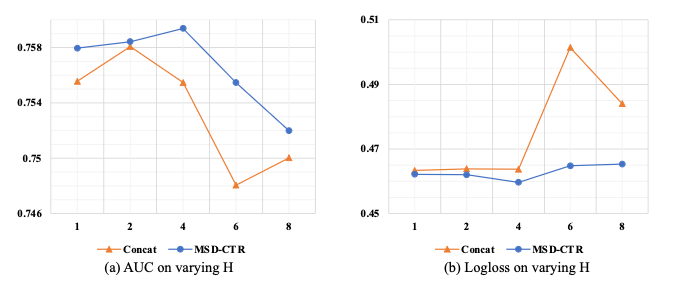
\includegraphics[width=\textwidth]{Figures/Chapter5/fig4.png}
    \caption{Performance comparison on different number of semantic views $H$ for MSD-CTR and Concat.}
    \label{fig:view-ablation}
\end{figure}

Results show that:
\begin{itemize}
    \item MSD-CTR benefits from disentangling semantic knowledge into multiple views, with optimal performance achieved at $H=4$ views.
    \item When $H$ becomes too large ($H \geq 6$), performance drops due to over-fragmentation of semantic information, leading to insufficient training data per view.
    \item Concat degrades faster as $H$ increases due to view overlap and multicollinearity, confirming the limitations of naive concatenation approaches.
    \item The performance gap between MSD-CTR and Concat increases with $H$, demonstrating the robustness of our disentanglement approach.
\end{itemize}

\textbf{Statistical Significance:} We conducted paired t-tests to verify the statistical significance of performance differences. With $p < 0.001$, the improvements are statistically significant across all view configurations.

\textbf{Computational Overhead:} While increasing $H$ improves semantic granularity, it also increases computational cost. Our analysis shows that $H=4$ provides the optimal trade-off between semantic understanding and computational efficiency for most practical applications.